% "Станет проще"

\documentclass[a4paper,12pt]{article} % тип документа

% report, book

% Си код
\usepackage{alltt}

% Рисунки
\usepackage{graphicx}
\usepackage{wrapfig}

\usepackage{hyperref}
\usepackage[rgb]{xcolor}
\hypersetup{				% Гиперссылки
    colorlinks=true,       	% false: ссылки в рамках
	urlcolor=blue          % на URL
}

%  Русский язык

\usepackage[T2A]{fontenc}			% кодировка
\usepackage[utf8]{inputenc}			% кодировка исходного текста
\usepackage[english,russian]{babel}	% локализация и переносы


% Математика
\usepackage{amsmath,amsfonts,amssymb,amsthm,mathtools} 


\usepackage{wasysym}

%Заговолок
\author{А.А. Хромов}
\title{Использование ассемблерных вставок в <<Си>> коде Hash table.}
\date{\today}



\begin{document} % начало документа

\maketitle
\newpage

\tableofcontents

\newpage

\section{Цель работы и материалы.}

Цель работы: написание эффективного кода, использующий хеш-тыблицы в работе со строками.\\
В работе используются: Xcode.
\section{Теоретическая часть}
В нашей программе будет использоваться 6 хеш-функций с номерами от 0 до 5:
\begin{alltt}
1	unsigned int Hash0 (char* str) \{
2	    return (int)(str [0]);
3	\}
\end{alltt}
Первая функция будет возвращать код первого символа в слове.
\begin{alltt}
1	unsigned int Hash1 (char* str) \{
2	    return 1;
3	\}
\end{alltt}
Вторая функция будет на любую строку возвращать 1.
\begin{alltt}
1	unsigned int Hash2 (char* str) \{
2	    return strlen(str);
3	\}
\end{alltt}
$\bigstar$Ну тут я считаю нужно крч задокументить, что эта делает: так как даже мне не очевидно. Окзаывается <<стрлен>> (есть оказывается такая функция, где-то в далеких стандартах <<Си>>, поэтому вы не пугайтесь) она, не буду тянуть, в общем, возвращает длину массива (в чарках).$\bigstar$
\begin{alltt}
1	unsigned int Hash3 (char* str) {
2	    int sum = 0;
3	    for (int i = 0; str [i] != 0; sum += str [i], i++) {}
4	    return sum;
5	}
\end{alltt}
Этот хеш суммирует все коды символов строки и возвращает её.
\begin{alltt}
1	unsigned int Hash4 (char* str) \{
2	    int h = 0;
3	    for (int i = 0; str [i] != 0; h = ((h << 5) + h) + str [i], i++) \{\}
4	    return h;
5	\}
\end{alltt}
GNU хеш, это вам не стрлен, тут все кристально понятно, если нет, то рекомендую ознакомиться с этим докладом позже, так как он может показаться вам сложными и не своевременным (замете, что <<тупым>> я вас не называл (вы сами это сделали в своей голове (мяу))).
\begin{alltt}
1	unsigned int Hash5 (char* str) \{
2	    unsigned int h = 0;
3	    
4	    for (int i = 0; str [i] != 0; i++) \{
5	        h = frol(h, 1) ^ str [i];
6	    \}
7	    return h;
8	\}
9
10	int frol (int n, int len) //ROL
11	\{
12	    if ((n % 2) == 1)
13	    \{
14	        return ((n << len) | 0x80);
15	    \}
16	    return n << len;
17	\}
\end{alltt}
Цикличекий сдвиг.
\\

Далее было бы целесообразно, рассказать некоторый <<геометрический>> смысл важных для нас функций, которые учавствуют в программе. Сам код будет выделен в приложении, или его можно будет найти в приложгающемся файле (А вообще вам должны были рассказать об этом на лекции и показать на семинаре, но если нет, то об этом очень внятно и коротко написано в <<кириченко>>, но лучше прочтитайте об этом в <<Сивухине>> (Мяу)).\\

И первое, нет это не мейн)), это функция 
\begin{alltt}
CraftString (list<char*>* array, int* size, unsigned int\\ (*Hash)(char*), int text_length, char* buf, const char*\\ name_files);
\end{alltt}
Она обрабатывает буфер <<char* buf>>, \underline{\textit{выделяет из него строку}}, и работает с ней по функции <<unsigned int (*Hash)(char*)>>, заполняя хеш-таблицу <<list<char*>* array>>, которую потом выводит в файл с именем <<const char* name\_files>>\\

Сама функция в работе со словом ссылается на другую функцию:
\begin{alltt}
int TablFind (list<char*>* array, char* str, int* size,\\ unsigned int (*Hash)(char*));
\end{alltt}
Она получает слово <<char* str>>, и отдает его уже в <<unsigned int\\ (*Hash)(char*)>>, после \underline{\textit{обрабатывает и заполняет хеш-таблицу}}\\\underline{\textit{<<list<char*>* array>> размера <<int* size>>}}.\\

На этом мы можем закончить поверхстное изучение основного кода, но хотелось бы так же заметить одну деталь, на которую мог обратить своё внимание "невнимательный" четатель. Мы использовали в работе свой класс <<list>> и о его устройстве тут, конечно же, рассказываться не будет, так как это выходит за рамки изучения оспекта проблемы (мне тупо лень Карл), о нем можно будет подробно узнать в приложении или в прилогающемся файле.
\section{Ход работы}

\subsection{Написание кода программы}

В работе нон-стоп пишем радостно код и паралленьно смотрим сериальчик, отвлекаясь на херстоун.\\
Пытаемся запустить код, а потом ещё раз и ещё. Удевительно, но факт: \textbf{\underline{\textit{ОН НЕ РАБОТАЕТ!!!}}}
\subsection{Написание кода программы ещё раз и правильно}

Тут совет от опытных пацанов с района: попробуйте выключить хотя бы игру, если результат повторится, то нужно будет так же выключить и сериальчек перед написанием кода.
\subsection{Сон}

Сон, а то вставать уже через 2 часа.
\subsection{Написание кода- что бы уже работал прям точно}

Ну вот, уже полдела сделано, можно показывать препу и поднять авторитет, что бы удос нам был прям обеспечен, но мы не станем. Давай те лучше вспомним цель нашей работы: <<Написание эффективного кода...>>. Прогоним наш код через профайл, и и снимем данные.

\begin{figure}[h!]
\begin{center}
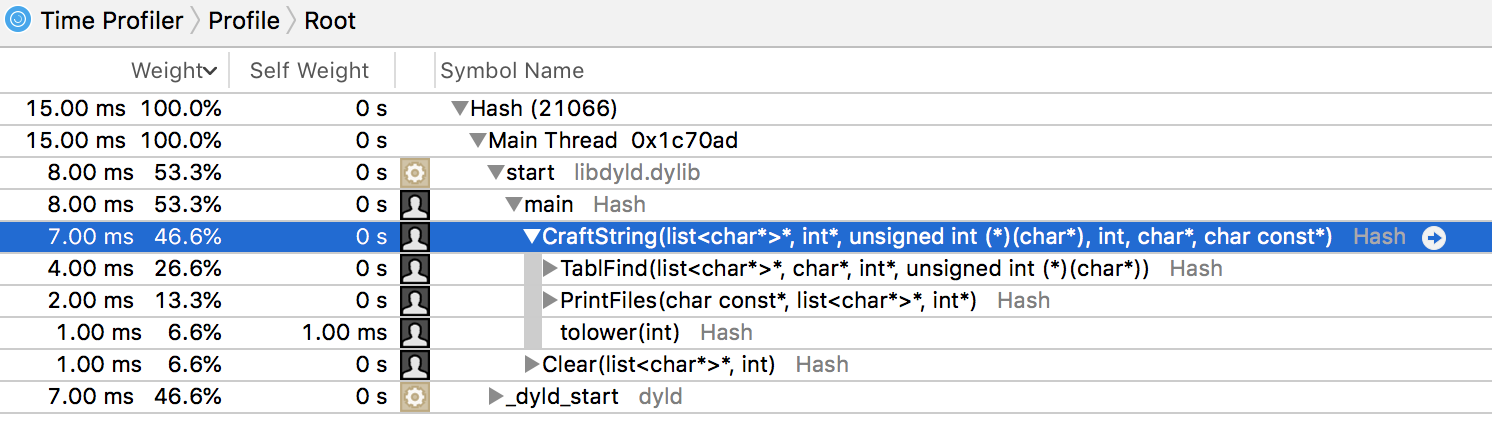
\includegraphics[width=1\textwidth]{1}
\end{center}
\caption{результаты profile для кода без асм. вставок.}
\end{figure}

Мы видим, что функции <<TablFind>> и <<PrintFiles>> "жрут" больше всего времени на выполнение. Рассмотрим вначале на вторую из них.

\begin{figure}[h!]
\begin{center}
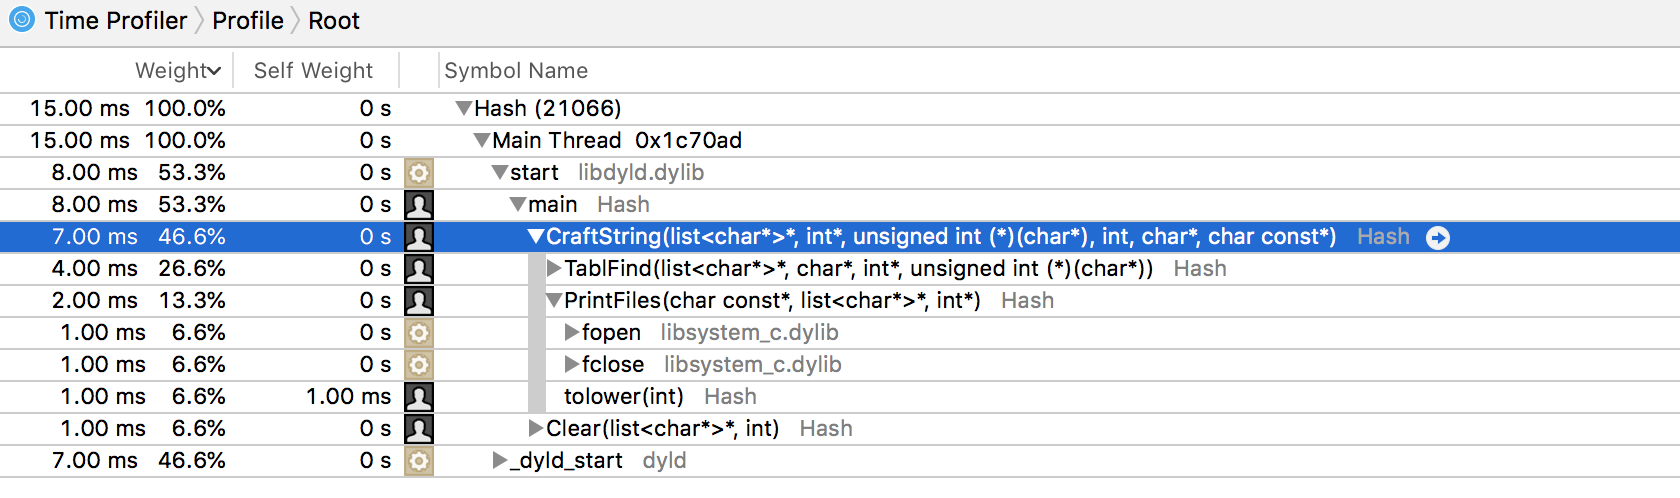
\includegraphics[width=1\textwidth]{2}
\end{center}
\caption{результаты profile для кода без асм. вставок.}
\end{figure}

И наблюдаем картину выполнения двух других функций <<fopen>>, <<fclose>>. Данные функции работают с файлами в которые записывают наши хеши. Работа с файлами всегда занимает много времени у процессора, поэтому оптимизировать эту область кода мы не можем.\\

Рассмотрим тогда первую функцию <<TablFind>>.\\
\newpage

\begin{figure}[h!]
\begin{center}
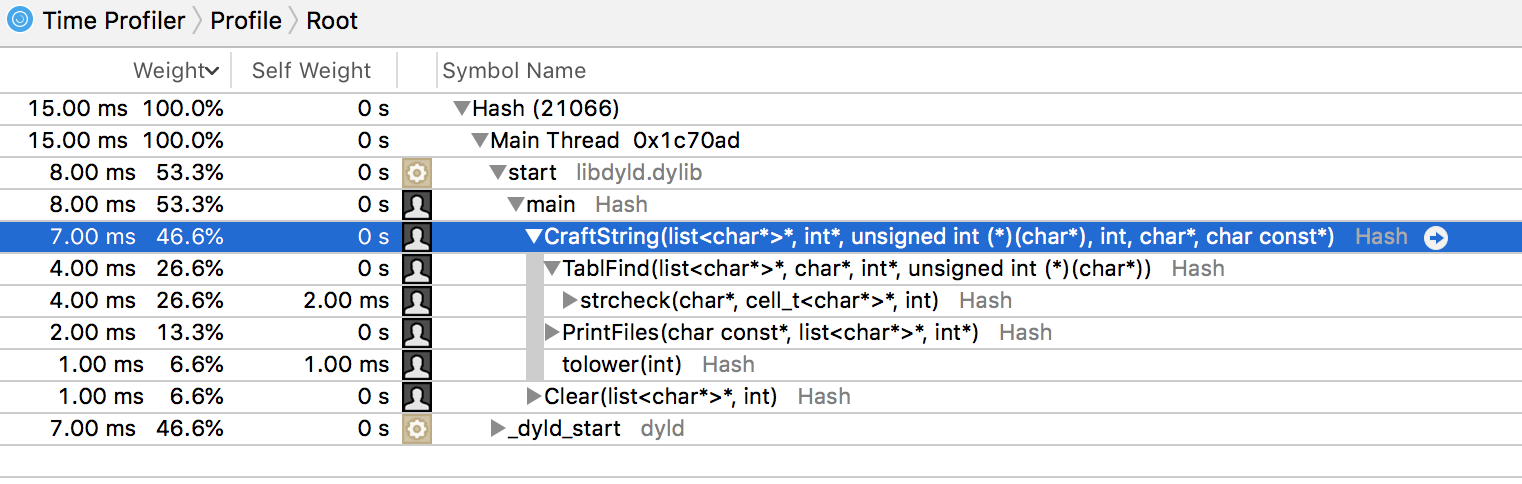
\includegraphics[width=1\textwidth]{3}
\end{center}
\caption{результаты profile для кода без асм. вставок.}
\end{figure}


Функция <<strcheck>> работает со строками, использует для этого команду strcmp. Предположив, что наш код мог бы обойтись без этой функции, он бы стал куда быстрее. Решим нашу проблему так же, как решали их наши деды. Вспомним язык древних канонов, язык высших созданий- машин, а именно несокрушимый и вечный \textbf{\underline{\textit{АССЕМБЛЕР!!!}}}

\begin{alltt}
1	bool strcheck(char* arg1, cell_t<char*>* cell, int size) \{
2	    int flag = 0;
3	    for (int j = 0; cell != nullptr; j++) \{
4	        
5	        flag = 0;
6	        \_\_asm\_\_ ("xor \%\%rax, \%\%rax              nt"
7	                 "L1:                           n"
8	                 "lodsb                         nt"
9	                 "test %%al, %%al               nt"
10	                 "jz EQU                        nt"
11	                 "xorb (%%rdi), %%al            nt"
12	                 "jnz EXIT                      nt"
13	                 "inc %%rdi                     nt"
14	                 "jmp L1                        nt"
15	                 "EQU:                          n"
16	                 "xorb (%%rdi), %%al            nt"
17	                 "EXIT:                         n"
18	                 "mov %%eax, %[x]               nt"
19	                 "nt"
20                  : [x] "=r" (flag)
21	                : [a] "S" (arg1), [b] "D" (cell->_data)
22                 :
23                 );
24        if (flag == 0)
25            return false;
26        cell = cell->_next;
27    \}
28    
29    return true;
30\}
\end{alltt}
Команда <<lodsb>> загрузить строковый операнд в AL.\\
Теперь наш код делает тоже самое, что и strcmp, но делает это намного быстрее, так как здесь отсутствует множество промежуточных опреаций с памятью, которые создаёт компилятор при работе с первоначальной функции.\\
Давайте прогоним код через <<profile>>:

\begin{figure}[h!]
\begin{center}
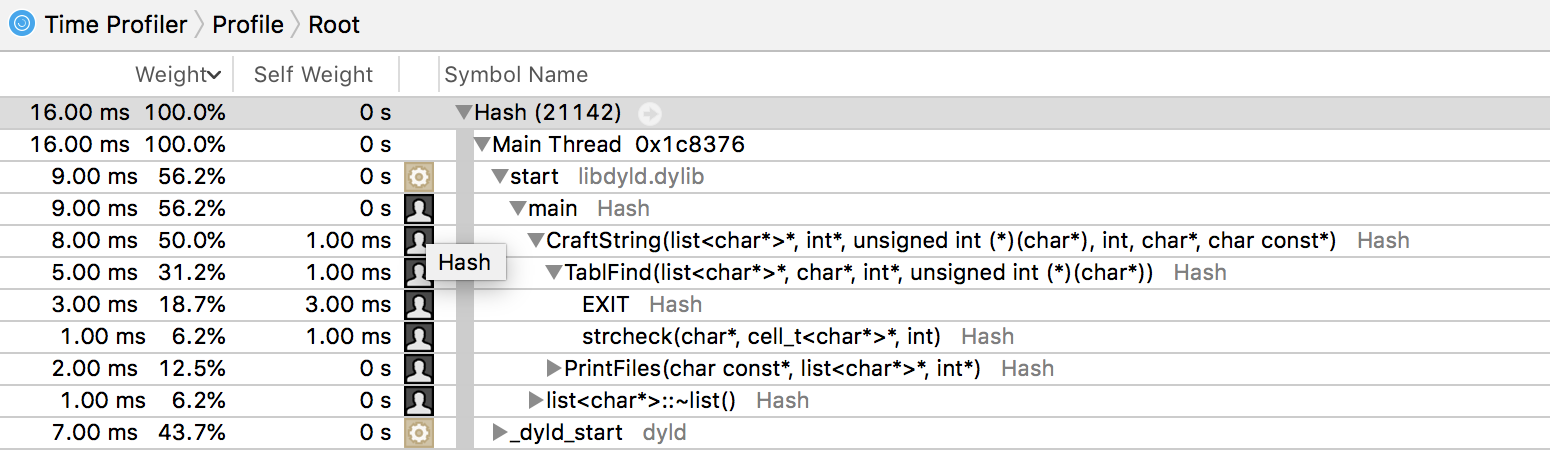
\includegraphics[width=1\textwidth]{41}
\end{center}
\caption{результаты profile для кода c асм. вставками.} \label{dz2}
\end{figure}

Результат на лицо, с 26\% до 6\% использования времени. В 4 раза сокращения времени спользование функции.

\section{Вывод.}
Мы написали эффективный код, использующий хеш-тыблицы в работе со строками, с помощью ассемблерных вставок, что дало спад использованного времени в 4 раза $\pm \varepsilon$.\\


\end{document}
